\chapter{Diseño de arquitectura de control}
\label{cap: diseno_arquitectura}

Este capítulo muestra el proceso de análisis, diseño e implementación de la arquitectura informática de control de la estación \acrshort{NPAM} robotizada. Se comenzará presentando el problema indicando aquellos aspectos considerados más importantes para los requisitos del sistema, para posteriormente describir el proceso de diseño que se ha seguido. Finalmente se presentará el desarrollo obtenido junto a un ejemplo de aplicación de una de sus funcionalidades. A partir del modelo de arquitectura presentado y el ejemplo de aplicación, se discutirán sus principales ventajas y aspectos por mejorar en nuevas iteraciones.

El código descrito en este capítulo se encuentra disponible en el repositorio GitHub del proyecto \cite{repo_github_TFM_MiguelLerinAlonso}. Los nodos de ROS2 que representan dichas tareas pertenecen al paquete \textit{rutine\_launcher}\footnote{Disponible en el direccionamiento: \textit{./workspace/ros\_ur\_driver/src/rutine\_launcher}}


\section{Introducción al problema}
La introducción de manipuladores robotizados en estaciones de fabricación aditiva supone el manejo de numerosas cantidades de datos y la abstracción de conceptos de robótica esenciales como pueden ser el cálculo de la cinemática, el muestreo de datos en directo del robot o la gestión del entorno de trabajo físico. Los robots colaborativos cuentan con su propia solución integrada dentro del manipulador, sin embargo, esta propuesta suele basarse en la gestión del \acrshort{PLC} acoplado al mismo y el conexionado a otras unidades. Es decir, no todo el mundo posee los conocimientos necesarios para poder operar dicho equipo y en ocasiones puede suponer un reto el conexionado de un nuevo sensor y la gestión de la información del robot.

Por estos motivos, se opta por integrar el manipulador robótico en un marco más grande donde existan unidades especializadas para cada una de la tareas antes mencionadas. Este marco suele enfocarse siempre a:

\begin{enumerate}
    \item Determinar unidades especializadas en las tareas clave del proceso de fabricación.
    \item Definir un conjunto de mensajes comunes a todos los elementos informáticos partícipes en el proceso.
    \item Construir un entorno modular que sea fácil de acceder y permita incorporar rápidamente nuevas funcionalidades.
\end{enumerate}

Teniendo en cuenta el marco de la estación con la que se está trabajando en este proyecto, la consecución de dichos objetivos debe pasar primero por una comprensión del flujo de trabajo que se desea implementar. A partir de dicho flujo será posible definir aquellas tareas más relevantes y asignar las responsabilidades que puede asumir el manipulador robótico por sí solo. Del mismo modo, dicha evaluación también servirá para identificar los puntos más críticos del proceso y evaluar si deben ser gestionados por otras unidades anexas.

\section{Metodología}
El procedimiento seguido en el este paquete de trabajo del proyecto puede dividirse en dos grandes etapas. La primera es la correspondiente a la definición de especificaciones y funcionalidades del proyecto, es decir, estudiar el flujo de trabajo del que parte la estación y definir sus requisitos y alcance del proyecto. La segunda etapa se da inmediatamente después de finalizar la primera y consta de la definición de todos los agentes automáticos que participan en el proceso de impresión \acrshort{NPAM} y cómo han de transmitirse mensajes entre unos y otros.

\subsection{Definición de especificaciones y funcionalidades}

En esta etapa se lleva una labor de estudio de las tecnologías \acrshort{AM} robotizadas y el estado de la técnica. Este estudio no se limita simplemente a la comprensión del flujo de trabajo convencional de este tipo de procesos, si no también del que se desea implementar en este proyecto y los antecedentes previos \cite{TFM_SanchoAmparo}\cite{TFM_Lu}.

Tal como se ha explicado en la sección \ref{section:  marco del proyecto}, este proyecto se encuentra integrado dentro de un entorno multidisciplinar más grande en el que cada equipo está especializado en una tarea del flujo de trabajo o en un elemento de la estación final. Esto es, el paso posterior al estudio descrito anteriormente fue ponerse en contacto con algunas de las distintas secciones del marco de trabajo para definir sus necesidades y discutir la información que necesitan o pueden aportar a este proyecto. 

Tomando como referencia la Figura \ref{fig:ambitos_coordinacion}, se estableció un diálogo con cada una de las secciones indicando el tipo de información que debían comunicarse entre sí y entre la sección representada por este proyecto. Del mismo modo, se estableció un alcance a aquellas informaciones que podían resultar relevantes para más de una sección. Aquellas secciones de mayor interés para esta tarea fueron:

\begin{itemize}
    \item \textbf{Generación de trayectorias:} Con esta sección se estuvo evaluando el proceso general de \textit{slicing} a partir de modelos \acrshort{CAD} de las piezas deseadas. Se describieron las limitaciones de cómputo y procesamiento que podía representar el proceso (número de puntos generados, tiempo de procesamiento, existencia de voladizos o representación entre distintos sistemas de referencia entre otros) y finalmente se acordó definir como resultado final del proceso un archivo CSV en el que se estableciese la trayectoria de impresión generada. Dicho archivo debía contener la posición y orientación de cada punto en un marco de referencia centrado en la base del robot manipulador.
    \item \textbf{Arquitectura:} La principal necesidad de esta sección era la definición de (1) un ecosistema software que permitiera realizar el cálculo de poses del cobot UR y (2) el conjunto de mensajes que debían ser procesados por una unidad central de cómputo a partir su \acrshort{PLC} integrado. Se acordó que el ecosistema software empleado estuviese fundamentado en ROS2 Humble, se utilizase la versión de Moveit correspondiente como principal controlador de cálculo de trayectorias robóticas y que Python fuese el lenguaje de programación de referencia (teniendo en cuenta el deseo de experimentar de forma rápida las nuevas trayectorias calculadas). También se incluyó la posibilidad de realizar una toma de datos del robot automatizada con parámetros relevantes como son las configuraciones articulares y la medida de entradas digitales o analógicas. En este último apartado un caso de empleo será la conexión del sensor láser SICK a una entrada del \acrshort{PLC}.
    \item \textbf{Actuadores máquina:} Los requisitos de este tipo de labores se basaban en (1) la integración de la cama de impresión diseñada en trabajos anteriores \cite{TFM_IñakiEchepare} con el cobot UR con capacidad para evitar la colisión con otros elementos de la estación y (2) proporcionar desde una unidad central las instrucciones de calentamiento de la plataforma de impresión (temperatura de consigna, sistema de regulación, alimentación eléctrica y protocolo de comunicaciones). Se acordó relacionar la plataforma de impresión con un armario de alimentación desarrollado por la sección de \textit{Diseño mecánico y eléctrico de la estación} y un microcontrolador programable que pudiese gestionar un circuito de control específicamente diseñado para regular la temperatura de la cama. De este modo, la plataforma de impresión podía suponer una herramienta más que se podía desacoplar rápidamente del sistema en caso de emergencia y además podía gestionarse a sí misma sin interferir con el resto de elementos.
\end{itemize}

Con las necesidades de los diferentes equipos definidas, se procedió a establecer una serie de guías de gestión de comunicaciones entre miembros de diversos equipos. Es decir, qué tipo de información podía ser más relevante para cada integrante dependiendo de su campo de trabajo. Estas indicaciones han sido descritas en la sección \ref{section:  marco del proyecto} con ayuda de la Figura \ref{fig:ambitos_coordinacion}.

\subsection{Flujo de trabajo y arquitectura}

Con las especificaciones y funcionalidades definidas, se dibuja una arquitectura informática que pueda solventar todas las necesidades antes expresadas. Es decir, se diseña un flujo de trabajo específico para esta estación evaluando las principales tareas, los equipos involucrados y los mensajes entre elementos de la arquitectura.

\subsubsection*{Flujo de trabajo}
\hypertarget{Flujo de trabajo arquitectura}{}
\bookmark[level=subsubsection,dest=Flujo de trabajo arquitectura]{Flujo de trabajo}

El flujo de trabajo empleado en esta estación se presenta en la Figura \ref{fig:tiempo_ciclo_estacion}. Este esquema representa las diferentes tareas del proceso utilizando un modelo de tiempo de ciclo parecido al de la Figura \ref{fig:tiempo_ciclo}. Dentro del proceso de fabricación aditiva se establecen tres etapas principales: \textit{Planificación}, \textit{Preparación} y \textit{Operación}.

\begin{figure}[h!]
    \centering
    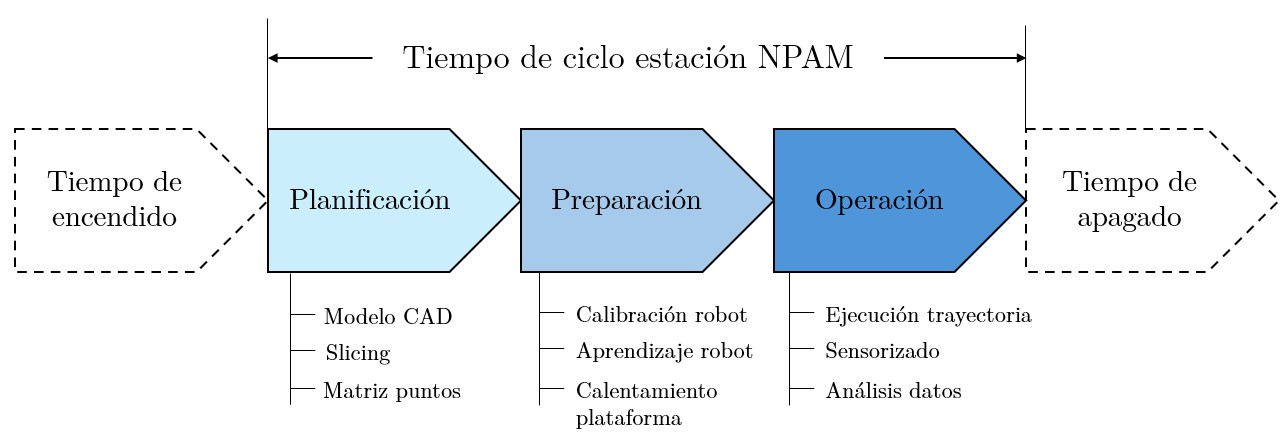
\includegraphics[scale=0.45]{figuras/tiempo_ciclo_estacion_v2.jpg}
    \caption{Flujo de trabajo expresado como tiempo de ciclo}
    \label{fig:tiempo_ciclo_estacion}
\end{figure}

Durante el tiempo de \textit{Planificación} se llevarán a cabo las tareas de diseño \acrshort{CAD} de la pieza a fabricar para que pase por un proceso de slicing. El resultado del slicer será un conjunto de puntos ordenados en el espacio en forma de matriz que representará cada ubicación exacta de deposición de material.

El tiempo de la fase de \textit{Preparación} se empleará en establecer, de forma previa a la ejecución del proceso de fabricación. los principales parámetros de control de la estación. Las operaciones clave de esta etapa se efectuarán en el siguiente orden: 
    \begin{enumerate}
        \item \textbf{Calibración del robot:} Para definir las relaciones entre los diferentes sistemas de referencia de la estación y la matriz de puntos obtenida de la etapa de \textit{Planificación}.
        \item \textbf{Aprendizaje del robot:} Para elaborar un conjunto de trayectorias y poses robotizadas a ejecutar. Dichas poses estarán enfocadas no solo en la deposición de material en los puntos indicados por la etapa de planificación, si no también en la gestión de riesgos de colisiones con otros elementos.
        \item \textbf{Calentamiento previo de la plataforma:} Comienza una vez que se haya validado que la trayectoria calculada es segura. Este proceso emitirá una señal de arranque de la operación en cuanto que se haya validado que la temperatura de la plataforma de impresión es la deseada y se mantiene estable.
    \end{enumerate}

El último tiempo es el de la etapa de \textit{Operación}, la cual comenzará una vez que se haya verificado la consecución completa de todas las tareas que conforman la \textit{Preparación}. En el transcurso de esta fase, el manipulador robótico efectuará la trayectoria calculada a través de los modelos de aprendizaje y se solicitará a una unidad de cómputo central el muestreo de datos de interés (posiciones, temperaturas, inercias del sistema, ...) Dichos datos podrán ser analizados en momentos posteriores con el objetivo de aportar mejoras sobre el proceso de fabricación y valorar su rendimiento.

\subsubsection*{Arquitectura}
\hypertarget{Arquitectura}{}
\bookmark[level=subsubsection,dest=Arquitectura]{Arquitectura}
La labor de diseño de la arquitectura informática se plantea teniendo en cuenta algunos de los aspectos planteados en la sección \ref{sec: arquitecturas_informaticas_estado_arte}, en la que se observó cómo aquellas soluciones que integran controladores especializados en diferentes tareas y niveles de abstracción han sido las de mayor éxito. Algunos de estos elementos especializados pueden ser la existencia de un controlador central, la disposición de una interfaz entre máquina y humano, el uso de varias capas de comunicaciones especializadas o un controlador exclusivo para el robot.

La Figura \ref{fig:arquitectura_TFM} muestra el diseño de arquitectura final realizado. Este diseño también sirve para definir el flujo de trabajo de la estación describiendo cinco grupos funcionales:
\begin{enumerate}
    \item \textbf{Slicer:} Elemento responsable de generar la trayectoria cartesiana de \textit{slicing} a partir del modelo \acrshort{CAD} de la pieza. Señalado en color rosa.
    \item \textbf{Computador central:} Señalado en color rojo, es el sistema informático que sirve de nexo entre el resto de elementos de la estación. Es el responsable de:
    \begin{itemize}
        \item Calcular los movimientos del robot a partir de las trayectorias del proceso de slicing.
        \item Operar el entorno de trabajo virtual del robot.
        \item Gestionar los mensajes del resto de grupos funcionales.
        \item Revisión de estado del resto de elementos.
    \end{itemize}
    \item \textbf{Plataforma de impresión:} Grupo funcional correspondiente a la gestión de la cama de impresión en cuanto a su control de temperatura y comunicaciones con el computador central. La gestión de estas tareas caen a cargo de una unidad de control que hace de interfaz entre el sistema de calentamiento de la cama y el resto de la estación. Todos sus componentes están coloreados en naranja.
    \item \textbf{Robot  UR:} Robot colaborativo responsable de recibir las trayectorias calculadas por el computador central. Este grupo funcional integra otras funcionalidades como aportar la calibración del robot y la toma provenientes de diferentes sensores conectados a su \acrshort{PLC}. Todos los equipos hardware y software que lo componen se identifican con el color amarillo.
    \item \textbf{Extrusor:} Sistema de control del extrusor de material de la estación. De forma análoga a la cama de impresión debe ser capaz de controlar automáticamente variables internas como son el flujo de material extruído, su temperatura o la corriente eléctrica demandada. Este grupo se identifica con el color verde claro.
\end{enumerate}

\begin{figure}[h!]
    \centering
    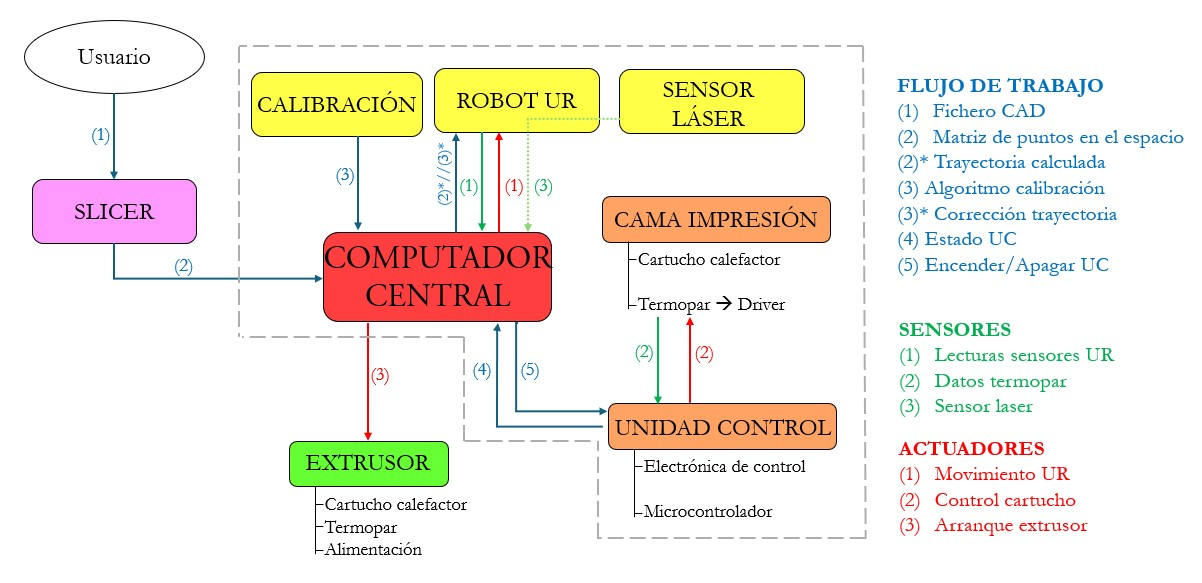
\includegraphics[scale=0.55]{figuras/arquitectura_TFM_v3.jpg}
    \caption{Arquitectura planteada en este proyecto}
    \label{fig:arquitectura_TFM}
\end{figure}

Por motivos de alcance del trabajo se toma que aquellos grupos funcionales en los que se trabajará son los encuadrados dentro de una línea de rayas gris en la Figura \ref{fig:arquitectura_TFM}. Es decir, en este proyecto sólo se tratarán los grupos funcionales del \textit{Computador central}, la \textit{Plataforma de impresión} y el \textit{Robot UR}. Los grupos funcionales de \textit{Slicer} y \textit{Extrusor} quedan a cargo de otros integrantes del marco de proyecto. 

Algunos elementos de los grupos funcionales describen otros componentes a un nivel de abstracción inferior. Por ejemplo es el grupo funcional del extrusor, que de forma análoga cuenta con un cartucho calefactor para el aporte de calor al sistema y un termopar como sensor de temperatura. Sin embargo, también efectúa otras funciones como la regulación del caudal de material de alimentación. Otro ejemplo, es el caso de la plataforma de impresión. Este grupo establece en la unidad de control un elemento regulador relé conectado a un microcontrolador que ha sido programado para regular su apertura a través de código. Por otra parte, la cama de impresión cuenta con un cartucho calefactor y un termopar que actúa como sensor de temperatura conectado al microcontrolador gracias a su propio driver..

Para la comunicación entre grupos funcionales se han definido mensajes especializados según el tipo de información que transcriben y la tarea dentro de la que se enmarcan. Los mensajes pueden referirse a información relacionada con el flujo de trabajo de la estación, la información de los sensores y las señales de activación de los actuadores.

Entre los mensajes relacionados con el flujo de trabajo de la estación (marcados en color azul en la Figura \ref{fig:arquitectura_TFM}) se encuentran:
\begin{itemize}
    \item \textbf{Fichero \acrshort{CAD}:} Modelo 3D diseñado por el usuario. Este modelo en formato \acrshort{STL} pasa a través del slicer para obtener el conjunto de puntos en el espacio donde se depositará el material extruído. 
    \item \textbf{Matriz de puntos en el espacio:} Es el resultado del slicing del modelo \acrshort{CAD} en forma de matriz. Estos puntos se sitúan sobre la plataforma de impresión y se referencian a un origen de coordenadas globales ubicado en la base del robot UR. Cada fila de la matriz representa a un único punto con posición cartesiana y orientación en forma de cuaternión unitario. Las tres primeras coordenadas del punto es la posición \textit{xyz} del punto, mientras que las cuatro últimas son las coordenadas \textit{ijkw} del cuaternión que indica la orientación. La Ecuación \ref{eq: punto_slicer} muestra un ejemplo de esta representación para el i-ésimo punto de la matriz.

    \begin{equation}
        \boldsymbol{p_i}= \begin{bmatrix}
            x_i & y_i & z_i & | & i_i& j_i& k_i& w_i 
        \end{bmatrix}
        \label{eq: punto_slicer}
    \end{equation}

    \item \textbf{Trayectoria  calculada:} La matriz de puntos elaborada en el proceso de slicing pasa al computador central, quien se responsabiliza de efectuar una lectura sobre ella y utilizar el controlador de ROS2 implementado para calcular su cinemática inversa. Esto es, se obtiene el conjunto de posiciones que debe adoptar el robot para alcanzar dichos puntos del espacio. Este mensaje se transmite al \acrshort{PLC} del robot para que su controlador integrado pueda aplicar dichos desplazamientos, se indica con el símbolo $(2)*$ para indicar que resulta del procesamiento directo de a través de ROS2 de la matriz de puntos. La definición explícita de este mensaje se indica en el capítulo \ref{cap: trayectorias}.

    \item \textbf{Algoritmo de calibración:} Es la parametrización de la calibración intrínseca del robot UR. Se define en formato \acrshort{YAML} indicando cómo se enlaza cada eslabón del robot con el siguiente y sus posiciones en el espacio. También se indican parámetros de interés como pueden ser los centros de inercia o el peso de cada eslabón. Este mensaje se inserta como un dato anexo que debe tener en cuenta la implementación ROS2 del computador central cuando se calcule la trayectoria articular.

    \item \textbf{Corrección de la trayectoria:} Trayectoria corregida gracias al controlador empleado dentro del controlador de ROS2 para tener en cuenta la calibración intrínseca del manipulador robótico y sus inercias, así como también los esfuerzos requeridos en cada articulación. Este mensaje se procesa en la implementación ROS2 del computador central de forma paralela a la trayectoria calculada, implementándose a modo de acción correctora sobre la misma. Esta relación entre ambos mensajes se indica con el símbolo $//$ para indicar un procesamiento paralelizado en el tiempo y $(3)*$ para resaltar que proviene de un procesamiento directo por parte de la implementación ROS2.

    \item \textbf{Estado de la Unidad de Control (UC):} Consigna de estado objetivo que debe alcanzar la unidad de control de temperatura de la cama de impresión. Este mensaje se manda directamente desde el computador central y es unidireccional, la responsabilidad de su correcto procesamiento recaerá sobre la unidad de control de la plataforma de impresión.

    \item \textbf{Encedido/Apagado de Unidad de Control (UC):} Mensaje de estado proporcionado por la propia unidad de control para indicar su activación y posibilidad de ejecución de trayectoria, así como un caso de apagado de emergencia.
\end{itemize}

Los mensajes relacionados con las señales de los sensores se indican en color verde en la Figura \ref{fig:arquitectura_TFM}, entre ellos destacan:
\begin{itemize}
    \item \textbf{Lectura de los sensores del manipulador UR:} Se sirven de la implementación ROS2 del computador central para proporcionar información constante de la configuración cinemática del robot (posiciones, velocidades y esfuerzos articulares). Estos datos se toman directamente desde el controlador \acrshort{PLC}, que hace de interfaz con los sensores internos del UR.

    \item \textbf{Datos del termopar:} Lectura de temperatura alcanzada en la cama de impresión. Esta información se procesa con un driver de lectura de dicho sensor y a continuación es integrada en el mensaje de Estado de la UC que se manda al computador central.

    \item \textbf{Sensor láser:} Medida de intensidad proporcionada por el sensor láser de la estación. Dicho sensor se conecta al \acrshort{PLC} del manipulador, por lo que se necesita implementar un sistema de lectura de entradas analógicas de dicho controlador con ROS2. Esta necesidad se ve representado con la línea de puntos verde que atraviesa el bloque de \textit{Robot UR} de la Figura \ref{fig:arquitectura_TFM}.
\end{itemize}

El color rojo corresponde a los mensajes de los actuadores que participan en la aquitectura informática de la Figura \ref{fig:arquitectura_TFM}. Estos mensajes son órdenes explícitas e inalterables que provienen del procesamiento de un controlador existente aguas arriba. Los más destacados son:
\begin{itemize}
    \item \textbf{Movimiento UR:} Orden de ejecución de movimiento del robot tomando como referencia la trayectoria calculada en el flujo de trabajo. Está comandada directamente desde el computador central.
    \item \textbf{Control del cartucho calefactor:} Mensaje que habilita la circulación de corriente a través del cartucho calefactor integrado dentro de la cama de impresión para aumentar su temperatura hasta el valor deseado. Buscando una mayor modularidad de la arquitectura, se decide que sea un mensaje gestionado únicamente desde la UC.
    \item \textbf{Arranque del extrusor:} Señal de arranque del mecanismo extrusor de material. Proviene desde el computador central y su definición queda fuera del alcance de este proyecto.
\end{itemize}


\section{Resultados y conclusiones}
Como resultado de la metodología implementada se expone un ejemplo de control general de la estación. En este caso se opta por la ejecución de una trayectoria robótica mientras se registran datos de las configuraciones cinemáticas adoptadas por el manipulador robótico haciendo uso del \acrshort{PLC} integrado y las posibilidades que ofrece ROS2 en este tipo de entornos. 

Dada la naturaleza mayor nivel de abstracción de este capítulo, este proceso se presenta como un ejemplo de los resultados obtenidos gracias a la metodología de diseño seguida. En posteriores capítulos se procederá a explicar de forma más concreta los fundamentos técnicos de cada una de las secciones de la arquitectura propuesta.

\subsection{Ejemplo de implementación}
\label{sec: ejemplo implementacion diseño arquitectura}

Se procede al cálculo y ejecución de una trayectoria sencilla para validar el correcto funcionamiento de las distintas unidades de la arquitectura y las comunicaciones que utilizan entre sí. El movimiento que debe seguir el \acrshort{TCP} del manipulador robótico se muestra en la Figura \ref{fig:trayectoria_objetivo}. Este movimiento cumple con las características definidas en trabajos de referencia para este proyecto \cite{paper_Q1_Alvaro_Adrian}\cite{TFM_SanchoAmparo}, y es el que se ha usado en los ensayos especializados para la validación de ejecución de trayectorias complejas y la calidad de la calibración introducida en el entorno de trabajo ROS2.  

Se trata de medio muelle de perfil cilíndrico que se fabrica depositando material sobre la cama de impresión. En capítulos posteriores se analizará con más detalle el desempeño del manipulador robótico junto al sistema de cálculo y ejecución cinemática, así como también la gestión de diferentes mensajes y la posibilidad de futuros análisis de datos.

\begin{figure}[h!]
    \centering
    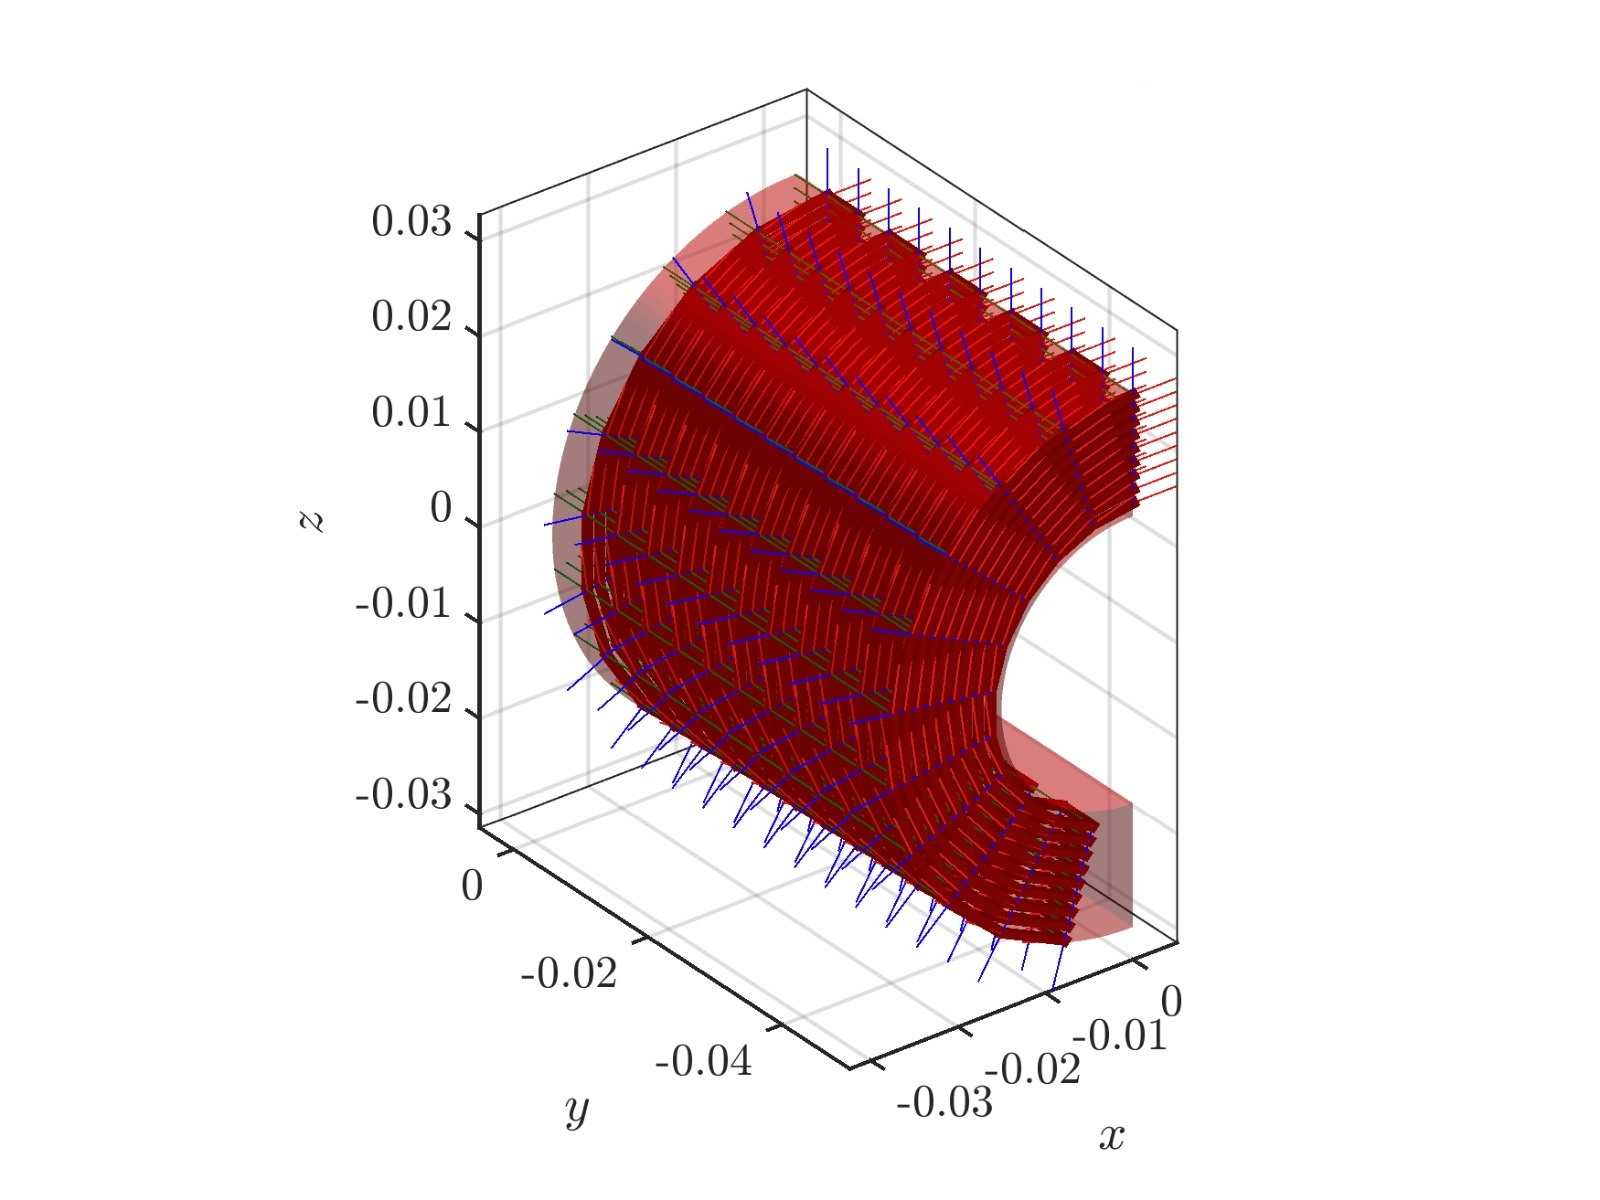
\includegraphics[scale=0.3]{figuras/trayectoria_objetivo.jpg}
    \caption{Trayectoria objetivo del ejemplo}
    \label{fig:trayectoria_objetivo}
\end{figure}

Se comienza arrancando el computador central e invocando una instancia del sistema de planificación offline. Este sistema se fundamenta en el empleo del controlador de ROS2 Moveit para las tareas de:

\begin{enumerate}
    \item Definición del espacio de trabajo.
    \item Imposición de restricciones de cálculo de trayectorias.
    \item Lectura de ficheros CSV de trayectoria objetivo resultado del proceso de slicing.
\end{enumerate}

Con estas tareas en mente se añade para este ejemplo una más: el muestreo de datos en directo relacionados con el desempeño del manipulador robótico durante la trayectoria efectuada.  

Con el entorno de trabajo virtualizado definido se abre una terminal que pueda establecer una comunicación directa con el manipulador. En el caso de este trabajo se opta por implementar un sistema basado en ROS2 que implemente el controlador cinemático Moveit. En otra terminal en paralelo, se accede invocar el nodo de ROS2 que llevará el grueso de la tarea. 

El procedimiento consiste en la invocación de un nodo perteneciente a un paquete de mayor nivel de abstracción conocido como \textit{rutine\_launcher}. El paquete \textit{rutine\_launcher}\footnote{Disponible en el repositorio del trabajo en la dirección:  \textit{./workspace/ros\_ur\_driver/src/rutine\_launcher/rutine\_launcher}} está enfocado en la definición y gestión de rutinas, es decir, la ejecución de nodos especializados en diversas tareas que trabajan bajo una estructura común. 

El nodo de este ejemplo combina el cálculo cinemático del manipulador, con el muestreo en directo de datos desde el \acrshort{PLC}. Este nodo se llama \textit{super\_logger\_launcher} y su funcionamiento se basa en la ejecución de instrucciones de ROS2 modulares, es decir, en la invocación síncrona de dos nodos. Un acercamiento a su forma de trabajar se aprecia en el pseudocódigo \ref{alg:algoritmo_super_logger_launcher}.


\begin{algorithm}[h!]
\caption{super\_logger\_launcher}\label{alg:algoritmo_super_logger_launcher}
\begin{algorithmic}[1]
\Require Entradas respectivas de los paquetes ROS2 especializados
\Ensure Ejecución de trayectoria simultánea al muestreo de datos UR
\State Definir la instrucción de invocación del nodo de cálculo y ejecución de cinemática
\State Definir la instrucción de invocación del nodo de muestreo de señales del PLC
\State Invocar una instancia del nodo de ejecución de trayectorias
\State Invocar una instancia del nodo de muestreo de señales PLC
\State Crear un suscriptor para el nodo de ejecución de trayectorias
\State Suscribir el nodo de muestreo de señales al suscriptor de las trayectorias

\If{Suscripción correcta}
    \State Cálculo de trayectoria
    \State Envío de señal de fin de cálculo de trayectoria a nodo de muestreo
    \If{Fin de cálculo de trayectoria == True}
        \State Ejecutar trayectoria
        \State Comenzar muestreo de datos
    \Else 
        \State Ejecutar trayectoria
        \State Mostrar error de muestreo
    \EndIf
\EndIf

\end{algorithmic}
\end{algorithm}

El algoritmo implementado se aprovecha de algunas características de los sistemas ROS como son la paralelización de procesos o el uso de comunicaciones síncronas entre los procesos del computador central. Para disminuir el grado de error se modifica la velocidad preestablecida en el entorno virtual para que se deje un pequeño margen de tiempo entre la señal de ejecución de trayectoria, el arranque del muestreado de datos y el comienzo del propio movimiento del robot. Esta velocidad se ha ajustado de forma estocástica ya que depende en gran medida del funcionamiento de la unidad integrada en la arquitectura.

\subsection{Resultados}
El robot es capaz de ejecutar la trayectoria encomendada por el nodo especialista en el cálculo de trayectorias de forma eficaz. Del mismo modo, es posible tomar un muestreo de las configuraciones cinemáticas de cada articulación del manipulador en tiempo real para posteriormente compararlas con las calculadas por el controlador ROS2 integrado en el sistema.

La Figura \ref{fig:ejemplo_muestreo} muestra el valor de cada posición articular calculada para la trayectoria  ensayada. Nótese cómo al tratarse de un movimiento rotativo de una articulación (la número 4 en este caso) mientras el resto permanecen prácticamente fijas, se observa que la articulación de giro sobre la que se apoya la plataforma de impresión muestra un trazado similar al de una señal sinusoidal. 

Por otro lado, el resto de articulaciones son las responsables de avanzar en el eje longitudinal de la cama y de variar en pequeños escalones la cota de impresión. Es decir mantienen un valor prácticamente constante en todo el tiempo de ejecución que solamente sufre correcciones periódicas en el momento de variar la altura de capa

\begin{figure}[h!]
    \centering
    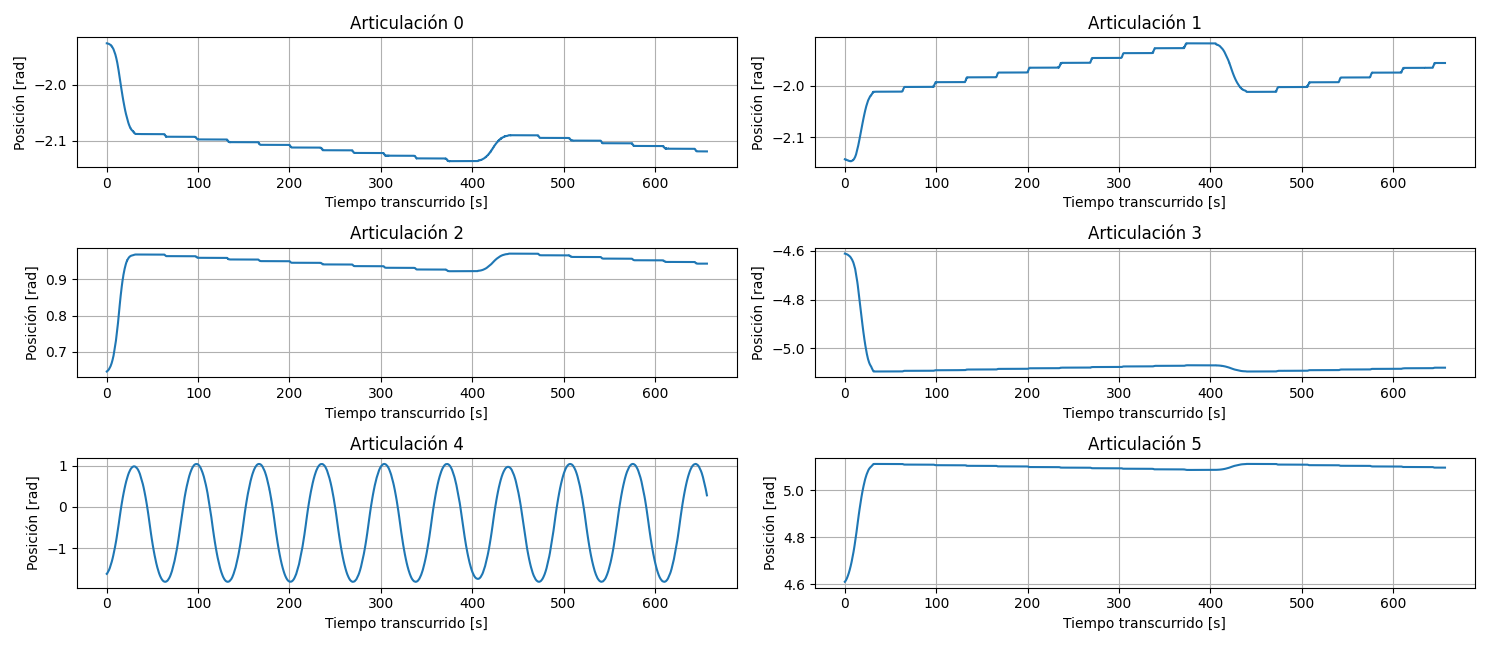
\includegraphics[scale=0.30]{figuras/ejemplo_muestreo.png}
    \caption{Posiciones articulares registradas durante el movimiento automático}
    \label{fig:ejemplo_muestreo}
\end{figure}

\subsection{Conclusiones}
Como se ha observado en el ejemplo de implementación, el sistema tiene capacidad para gestionar tareas complejas con relativa facilidad. Es decir, el computador central puede adaptar el tipo de mensaje que necesita cada unidad especializada para que sea ejecutado con precisión y teniendo en cuenta el entorno de trabajo real en el que se mueve el manipulador robótico.

La presencia de módulos especializados favorece la inserción de nuevos dispositivos al sistema, como puede ser en este caso el sensor láser o la lectura directa del \acrshort{PLC}. Tanto la lectura de datos como la ejecución de trayectorias se hacen utilizando como base la interfaz de programación dispuesta por ROS2. Es decir, se facilita la labor de validación de trayectorias siguiendo fundamentalmente la filosofía del aprendizaje offline.
No obstante. la capacidad de toma de datos directa del manipulador también favorece introducir una parte de aprendizaje online, dejando siempre libre la posibilidad de registrar un movimiento del cobot guiado por el operario a partir del cual generar una nueva trayectoria. 

De igual modo, la interfaz introducida en el paquete de lanzamiento de rutinas, facilita la definición de paquetes más sencillos con los parámetros deseados por el operario, dejando un control total sobre aspectos que se describirán con más detalle en los siguientes capítulos como pueden ser el número de muestras, la temperatura de calentamiento de la cama o la velocidad de ejecución del movimiento. Esto es, se realiza una gestión de las comunicaciones entre diferentes unidades funcionales utilizando los conceptos aportados por el entorno de trabajo ROS2, cuyo grafo de conexionado completo se puede consular en el anexo \ref{cap: anexo grafos nodos ros2}.